
\hypertarget{introduction}{%
\section{Introduction}\label{introduction}}

Writing programs (or programming) is a very creative and rewarding activity. You can write programs for many reasons, ranging from making your living to solving a difficult data analysis problem to having fun to helping someone else solve a problem. This book assumes that \emph{everyone} needs to know how to program, and that once you know how to program you will figure out what you want to do with your newfound skills.

We are surrounded in our daily lives with computers ranging from laptops to cell phones. We can think of these computers as our "personal assistants" who can take care of many things on our behalf. The hardware in our current-day computers is essentially built to continuously ask us the question, ``What would you like me to do next?''.

Programmers add an operating system and a set of applications to the hardware and we end up with a Personal Digital Assistant that is quite helpful and capable of helping us do many different things.

Our computers are fast and have vast amounts of memory and could be very helpful to us if we only knew the language to speak to explain to the computer what we would like it to "do next". If we knew this language, we could tell the computer to do tasks on our behalf that were repetitive. Interestingly, the kinds of things computers can do best are often the kinds of things that we humans find boring and mind-numbing.

For example, look at the first three paragraphs of this chapter and tell me the most commonly used word and how many times the word is used. While you were able to read and understand the words in a few seconds, counting them is almost painful because it is not the kind of problem that human minds are designed to solve. For a computer, the opposite is true, reading and understanding text from a piece of paper is hard for a computer to do, but counting the words and telling you how many times the most used word was used is very easy for a computer.

\begin{Verbatim}[frame=single]
>>> python words.py
  Write the name of the text file: first-3-paragraphs.txt
  The word is: 'to'
  It appears 11 times
\end{Verbatim}

Our ``personal information analysis assistant'' quickly told us that the word ``to'' was used eleven times in the first three paragraphs of this chapter.

This very fact that computers are good at things that humans are not is why you need to become skilled at talking ``computer language''. Once you learn this new language, you can delegate mundane tasks to your partner (the computer), leaving more time for you to do the things that you are uniquely suited for. You bring creativity, intuition, and inventiveness to this partnership.

To execute a task or solve a problem we use algorithms. 
\begin{definition}
An \textbf{algorithm} is a sequence of specific instructions of the actions to be performed and in what order to complete a given task.
\end{definition}

For example, a recipe for cooking paella is like an algorithm that consists of a sequence of steps that you have to follow to cook paella.
%
Other algorithms that we know, for example, are the steps we learn in school to multiply (see Figure \ref{fig:multiplicar}). 

\begin{figure}
    \centering
    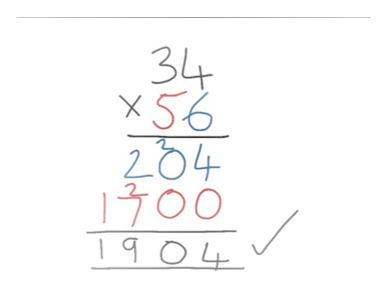
\includegraphics[width=0.5\textwidth]{images/multiplicar}
    \caption{Algorithm for multiplying 34 by 56}
    \label{fig:multiplicar}
\end{figure}


\begin{itemize}[nosep]
\item
  step 1: we put the multiplicand (34) above and the multiplier (56) below
\item
  step 2: multiply the units of the multiplier by the multiplicand and write the result in the row below.
\item
  step 3: multiply the tens of the multiplier by the multiplicand and write the result in the bottom row but shifted one position to the left.
\item
  step 4: sum the two products
\end{itemize}

\hypertarget{arquitectura-hardware-de-los-ordenadores}{%
\section{Computer hardware architecture}\label{arquitectura-hardware-de-los-ordenadores}}

\index{hardware} \index{hardware!arquitectura}

Before we start learning the language we speak to give instructions to computers to develop software, we need to learn a small amount about how computers are built. If you were to take apart your computer or cell phone and look deep inside, you would find different components that can be seen in Figure \ref{fig:arch}.

\begin{figure}
    \centering
    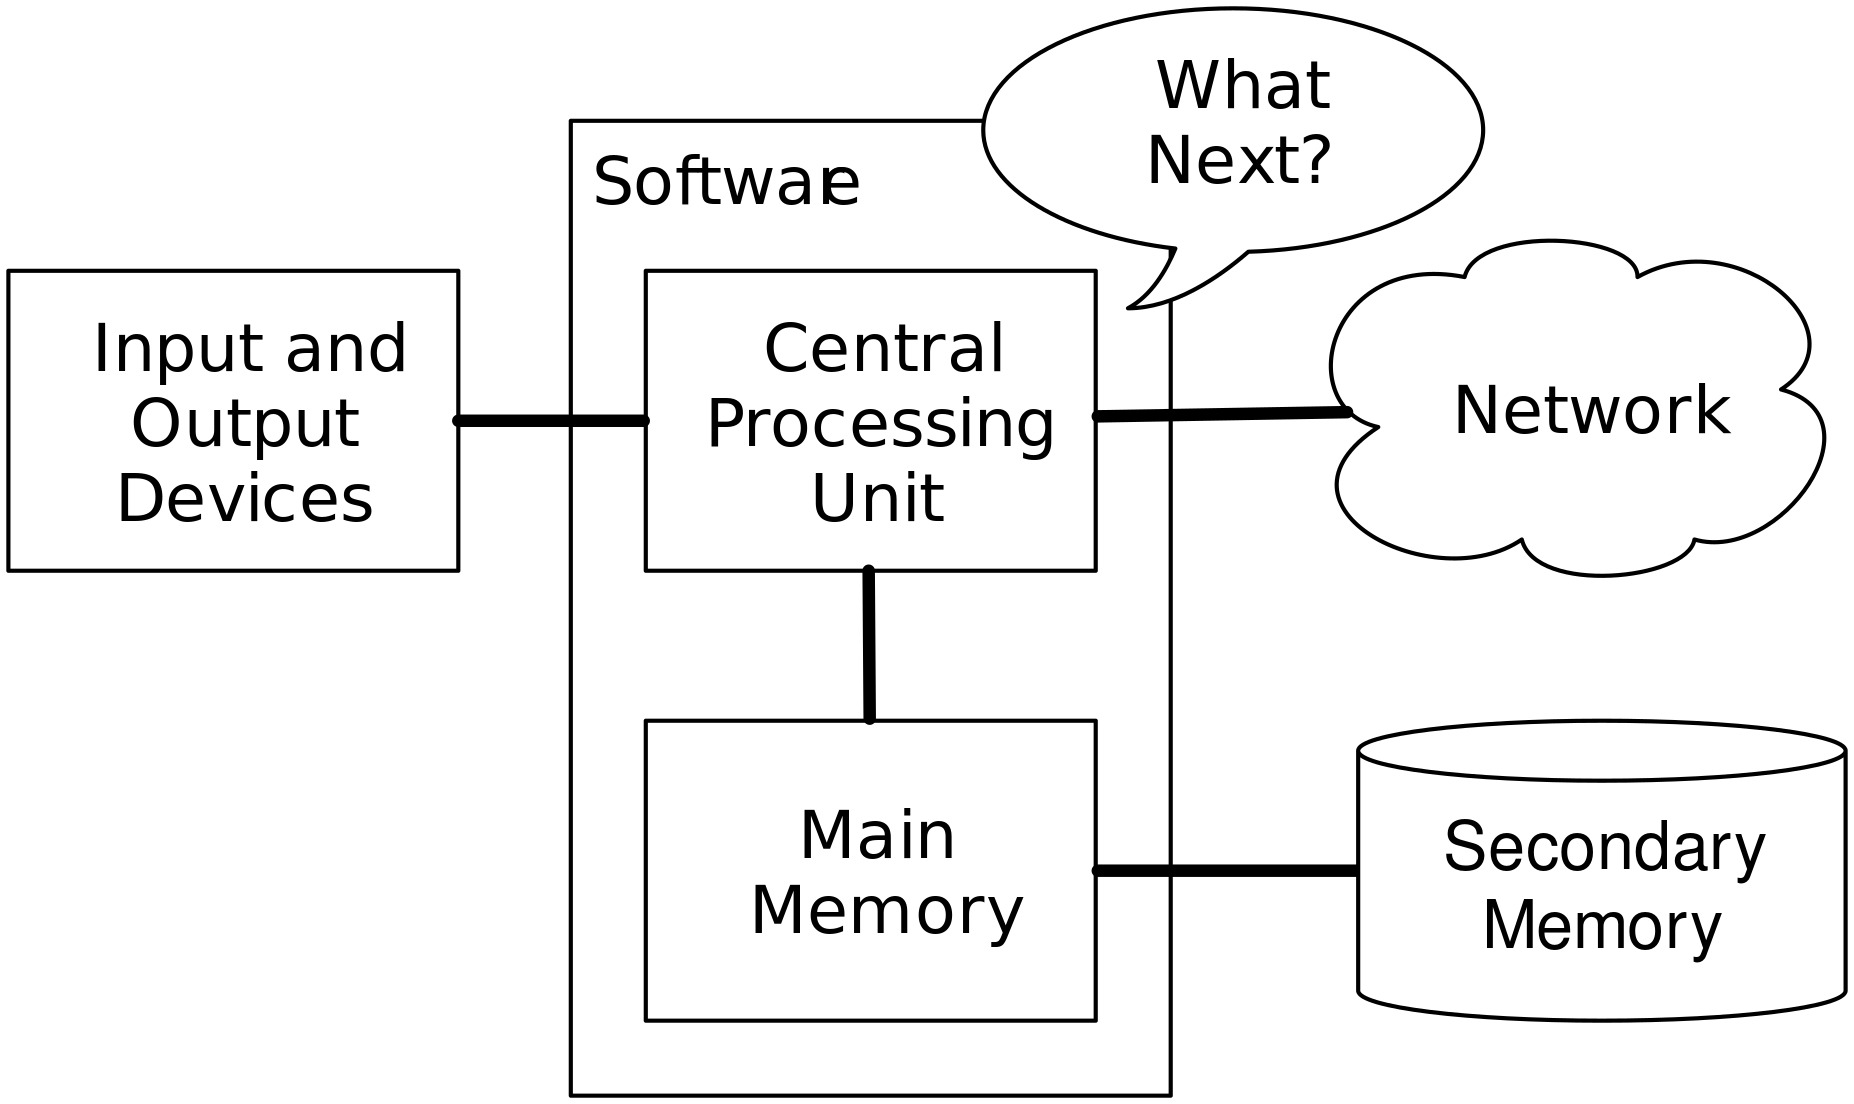
\includegraphics[width=0.5\textwidth]{images/comp-hw-arch.jpg}
    \caption{Computer hardware architecture}
    \label{fig:arch}
\end{figure}


The high-level definitions of these parts are as follows:

\begin{itemize}[nosep]
\item
  The \emph{Central Processing Unit} (or CPU) is the part of the computer that is built to be obsessed with "what is next?" If your computer is rated at 3.0 Gigahertz, it means that the CPU will ask "What next?" three billion times per second. You are going to have to learn how to talk fast to keep up with the CPU.
\item
  The \emph{Main Memory} is used to store information that the CPU needs in a hurry. The main memory is nearly as fast as the CPU. But the information stored in the main memory vanishes when the computer is turned off.
\item
  The \emph{Secondary Memory} is also used to store information, but it is much slower than the main memory. The advantage of the secondary memory is that it can store information even when there is no power to the computer. Examples of secondary memory are disk drives or flash memory (typically found in USB sticks and portable music players).
\item
  The \emph{Input and Output Devices} are simply our screen, keyboard, mouse, microphone, speaker, touchpad, etc. They are all of the ways we interact with the computer.
\item
  These days, most computers also have a \emph{Network Connection} to retrieve information over a network. We can think of the network as a very slow place to store and retrieve data that might not always be ``up''. So in a sense, the network is a slower and at times unreliable form of \emph{Secondary Memory}.
\end{itemize}

While most of the detail of how these components work is best left to computer builders, it helps to have some terminology so we can talk about these different parts as we write our programs.

As a programmer, your job is to use and orchestrate each of these resources to solve the problem that you need to solve and analyze the data you get from the solution. As a programmer you will mostly be "talking" to the CPU and telling it what to do next. Sometimes you will tell the CPU to use the main memory, secondary memory, network, or the input/output devices.

\begin{figure}
\centering
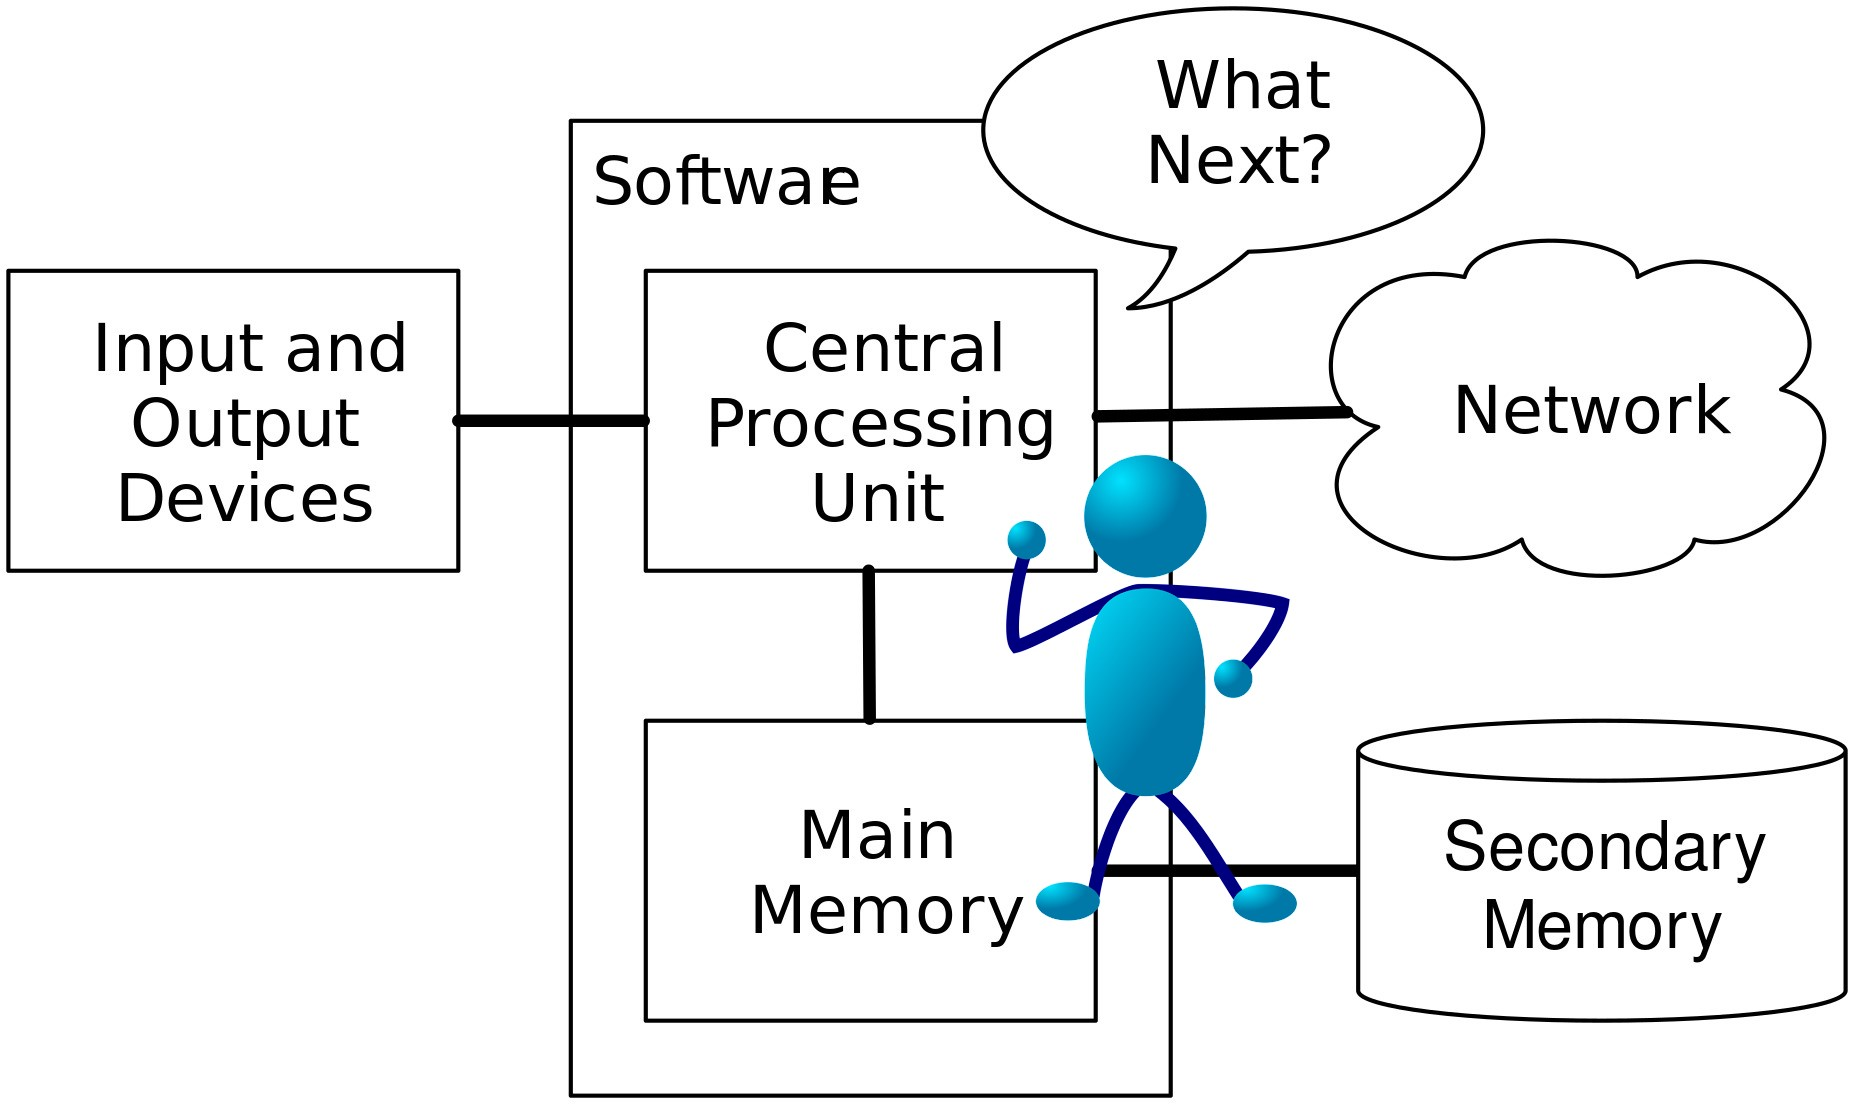
\includegraphics[width=0.5\textwidth]{images/comp-hw-arch-2.jpg}
\caption{Where are you as a programmer?}
\label{fig:donde-estas}
\end{figure}

You need to be the person who answers the CPU's "What next?" question. But it would be very uncomfortable to shrink you down to 5mm tall and insert you into the computer just so you could issue a command three billion times per second. So instead, you must write down your instructions in advance. We call these stored instructions a \emph{program} and the act of writing these instructions down and getting the instructions to be correct \emph{programming}.

\hypertarget{programation}{%
\section{Understanding programming}\label{programation}}

Creating useful and smart programs for others to use is a very creative activity. Programming is the discipline related to:

\begin{itemize}[nosep]
\item
  Problem solving using algorithms
\item
  Code the algorithm as a program in a certain language
\item
  Test the program by running it with the computer
\end{itemize}

In this subject, we will try to turn you into a person who is skilled in the art of programming. In the end you will be a \emph{programmer} - perhaps not a professional programmer, but at least you will have the skills to look at a data/information analysis problem and develop algorithms/programs to solve the problem.

\index{resolución de un problema}

In a sense, you need two skills to be a programmer:

\begin{itemize}[nosep]
\item
  First, you need to know the programming language (Python) - you need to know the vocabulary and the grammar. You need to be able to spell the words in this new language properly and know how to construct well-formed ``sentences'' in this new language.
\item
  Second, you need to ``tell a story''. In writing a \emph{story}, you combine words and sentences to convey an \emph{idea} to the reader. There is a skill and art in constructing the story, and skill in story writing is improved by doing some writing and getting some feedback. In programming, our \emph{algorithm} is the ``story'' and the \emph{problem} you are trying to solve is the ``idea''.
\item
  Third, you need to verify that the reader interprets your story well so that there are no misunderstandings. In programming that means we have to run {\em tests} with our program, to ensure that it does what we want it to do.
\end{itemize}

Once you learn one programming language such as Python, you will find it much easier to learn a second programming language such as JavaScript or C++. The new programming language has very different vocabulary and grammar but the problem-solving skills will be the same across all programming languages.

You will learn the ``vocabulary'' and ``sentences'' of Python pretty quickly. It will take longer for you to be able to write a coherent program to solve a brand-new problem. We teach programming much like we teach writing. We start reading and explaining programs, then we write simple programs, and then we write increasingly complex programs over time. At some point you ``get your muse'' and see the patterns on your own and can see more naturally how to take a problem and write a program that solves that problem. And once you get to that point, programming becomes a very pleasant and creative process.

We start with the vocabulary and structure of Python programs.

\hypertarget{palabras-y-frases}{%
\section{Words and sentences}\label{palabras-y-frases}}

\index{lenguaje de programación} \index{lenguaje!programación}

Unlike human languages, the Python vocabulary is actually pretty small. We call this ``vocabulary'' the ``reserved words''. These are words that have very special meaning to Python. When Python sees these words in a Python program, they have one and only one meaning to Python. Later as you write programs you will make up your own words that have meaning to you called \emph{variables}. You will have great flexibility in choosing your names for your variables, but you cannot use any of Python's reserved words as a name for a variable.

When we train a dog, we use special words like ``sit'', ``stay'', and ``fetch''. When you talk to a dog and don't use any of these special words, they just look at you with a quizzical look on their face until you say a special word. For example, if you say, "I wish more people would walk to improve their overall health", what most dogs likely hear is, "blah blah blah \emph{walk} blah blah blah blah." That is because "walk" is a reserved word in dog language. Many might suggest that the language between humans and cats has no reserved words\footnote{\url{http://xkcd.com/231/}}.

The reserved words in the language where humans talk to Python include the following:

\begin{verbatim}
and       del       global      not       with
as        elif      if          or        yield
assert    else      import      pass      
break     except    in          raise
class     finally   is          return
continue  for       lambda      try
def       from      nonlocal    while    
\end{verbatim}

That is it, and unlike a dog, Python is already completely trained. When you say ``try'', Python will try every time you say it without fail\footnote{The word ``try'' is also a reserved word within the
Python language.}.

We will learn these reserved words and how they are used in the future, but for now we will focus on the Python equivalent of ``speak'' (in human-to-dog language). The nice thing about telling Python to speak is that we can even tell it what to say by giving it a message in quotes:

\begin{Verbatim}[frame=single]
    print('Hello, world!')
\end{Verbatim}

And we have even written our first syntactically correct Python sentence. Our sentence starts with the function \emph{print} followed by a string of text of our choosing enclosed in single quotes. The strings in the print statements are enclosed in quotes. Single quotes and double quotes do the same thing; most people use single quotes except in cases like this where a single quote (which is also an apostrophe) appears in the string.

\section{Installing Thonny, an integrated development environment (IDE)}

Before you can converse with Python, you will need to install the necessary software on your computer and learn how to start Python on it. In this course we use {\em Thonny} (\url{https://thonny.org/}), an integrated development environment (IDE) designed for beginners. It is easy to use, consumes few resources and also incorporates the Python version 3 interpreter.


The Thonny screen has incorporates some windows. This presentation is configurable but most of the time we will use the layout seen in Figure~\ref{fig:Thonny} and which we will explain below.

\begin{figure}
	\centering
	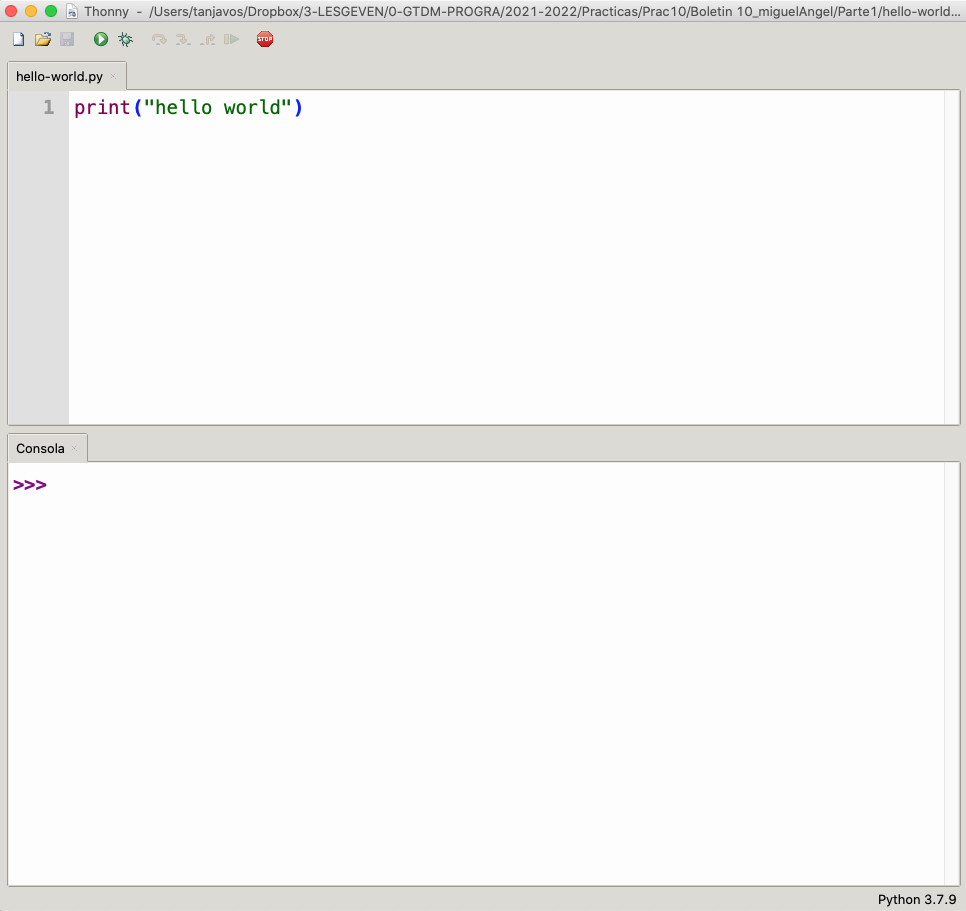
\includegraphics[width=.85\textwidth]{images/Thonny.png}
	\caption{Thonny interface}
	\label{fig:Thonny}
\end{figure}

At the top we find different buttons to, for example, open, run and stop programs.

Below that, we find the main work windows:

\begin{itemize}[nosep]
 \item the code editor where we can create and edit our programs.
 \item the shell or launch console is located below. Through it, we can converse with Python and our programs, either by entering data or seeing the results that it presents. It will also allow us to interactively execute Python commands.
 
 The \verb|>>>| prompt is the Python interpreter's way of asking you, ``What do you want me to do next?'' Python is ready to have a conversation with you. All you have to know is how to speak the Python language.
\end{itemize}


\hypertarget{conversando-con-python}{%
\section{Conversing with Python}\label{conversando-con-python}}


Let's say for example that you did not know even the simplest Python language words or sentences. You might want to use the standard line that astronauts use when they land on a faraway planet and try to speak with the inhabitants of the planet:

\begin{Verbatim}[frame=single]
>>> I come in peace, please take me to your leader
      File "<stdin>", line 1
        I come in peace, please take me to your leader
             ^
    SyntaxError: invalid syntax
>>>
\end{Verbatim}


This is not going so well. Unless you think of something quickly, the inhabitants of the planet are likely to stab you with their spears, put you on a spit, roast you over a fire, and eat you for dinner.

Luckily you brought a copy of this book on your travels, and you thumb to this very page and try again:

\begin{Verbatim}[frame=single]
>>> print('Hello world!')
    Hello world!
\end{Verbatim}

This is looking much better, so you try to communicate some more:

\begin{Verbatim}[frame=single]
>>> print('You must be the legendary god that comes from the sky')
    You must be the legendary god that comes from the sky
>>> print('We have been waiting for you for a long time')
    We have been waiting for you for a long time
>>> print('Our legend says you will be very tasty with mustard')
    Our legend says you will be very tasty with mustard
>>> print 'print 'We will have a feast tonight unless you say
    File "<stdin>", line 1
        print 'print 'We will have a feast tonight unless you say
                                                                ^
    SyntaxError: Missing parentheses in call to 'print'
    >>>
\end{Verbatim}

The conversation was going so well for a while and then you made the tiniest mistake using the Python language and Python brought the spears back out.

At this point, you should also realize that while Python is amazingly complex and powerful and very picky about the syntax you use to communicate with it, Python is not intelligent. You are really just having a conversation with yourself, but using proper syntax.

In a sense, when you use a program written by someone else the conversation is between you and those other programmers with Python acting as an intermediary. Python is a way for the creators of programs to express how the conversation is supposed to proceed. And in just a few more chapters, you will be one of those programmers using Python to talk to the users of your program.

Before we leave our first conversation with the Python interpreter, you should probably know the proper way to say ``good-bye'' when interacting with the inhabitants of Planet Python:

\begin{Verbatim}[frame=single]
>>> good-bye
    Traceback (most recent call last):
      File "<stdin>", line 1, in <module>
    NameError: name 'good' is not defined
>>> if you don't mind, I need to leave
      File "<stdin>", line 1
        if you don't mind, I need to leave
                 ^
    SyntaxError: invalid syntax
>>> quit()
\end{Verbatim}

You will notice that the error is different for the first two incorrect attempts. The second error is different because \emph{if} is a reserved word and Python saw the reserved word and thought we were trying to say something but got the syntax of the sentence wrong.

The proper way to say ``good-bye'' to Python is to enter \emph{quit()} at the interactive chevron
\texttt{\textgreater{}\textgreater{}\textgreater{}} prompt. It would have probably taken you quite a while to guess that one, so having a book handy probably will turn out to be helpful.

\hypertarget{terminologuxeda-intuxe9rprete-y-compilador}{%
\section{Terminology: interpreter and
compiler}\label{terminologuxeda-intuxe9rprete-y-compilador}}

Python is a \emph{high-level} language intended to be relatively straightforward for humans to read and write and for computers to read and process. Other high-level languages include Java, C++, PHP, Ruby, Basic, Perl, JavaScript, and many more. The actual hardware inside the Central Processing Unit (CPU) does not understand any of these high-level languages.

The CPU understands a language we call \emph{machine language}. Machine language is very simple and frankly very tiresome to write because it is represented all in zeros and ones:

\begin{verbatim}
    001010001110100100101010000001111
    11100110000011101010010101101101
    ...
\end{verbatim}

Machine language seems quite simple on the surface, given that there are only zeros and ones, but its syntax is even more complex and far more intricate than Python. So very few programmers ever write machine language. Instead we build various translators to allow programmers to write in high-level languages like Python or JavaScript and these translators convert the programs to machine language for actual execution by the CPU.

Since machine language is tied to the computer hardware, machine language is not \emph{portable} across different types of hardware. Programs written in high-level languages can be moved between different computers by using a different interpreter on the new machine or recompiling the code to create a machine language version of the program for the new machine.

These programming language translators fall into two general categories: (1) interpreters and (2) compilers.

An interpreter reads the source code of the program as written by the programmer, parses the source code, and interprets the instructions on the fly. Python is an interpreter and when we are running Python interactively, we can type a line of Python (a sentence) and Python processes it immediately and is ready for us to type another line of Python.

Some of the lines of Python tell Python that you want it to remember some value for later. We need to pick a name for that value to be remembered and we can use that symbolic name to retrieve the value later. We use the term \emph{variable} to refer to the labels we use to refer to this stored data.

\begin{Verbatim}[frame=single]
>>> x = 6
>>> print(x)
  6
>>> y = x * 7
>>> print(y)
  42
>>>
\end{Verbatim}
In this example, we ask Python to remember the value six and use the label \emph{x} so we can retrieve the value later. We verify that Python has actually remembered the value using \emph{print}. Then we ask Python to retrieve \emph{x} and multiply it by seven and put the newly computed value in \emph{y}. Then we ask Python to print out the value currently in \emph{y}.

Even though we are typing these commands into Python one line at a time, Python is treating them as an ordered sequence of statements with later statements able to retrieve data created in earlier statements. We are writing our first simple paragraph with four sentences in a logical and meaningful order.

It is the nature of an \emph{interpreter} to be able to have an interactive conversation as shown above. A \emph{compiler} needs to be handed the entire program in a file, and then it runs a process to translate the high-level source code into machine language and then the compiler puts the resulting machine language into a file for later execution.

If you have a Windows system, often these executable machine language programs have a suffix of ``.exe'' or ``.dll'' which stand for ``executable'' and ``dynamic link library'' respectively. In Linux and Macintosh, there is no suffix that uniquely marks a file as executable.

If you were to open an executable file in a text editor, it would look completely crazy and be unreadable:

\begin{verbatim}
    ^?ELF^A^A^A^@^@^@^@^@^@^@^@^@^B^@^C^@^A^@^@^@\xa0\x82
    ^D^H4^@^@^@\x90^]^@^@^@^@^@^@4^@ ^@^G^@(^@$^@!^@^F^@
    ^@^@4^@^@^@4\x80^D^H4\x80^D^H\xe0^@^@^@\xe0^@^@^@^E
    ^@^@^@^D^@^@^@^C^@^@^@^T^A^@^@^T\x81^D^H^T\x81^D^H^S
    ^@^@^@^S^@^@^@^D^@^@^@^A^@^@^@^A\^D^HQVhT\x83^D^H\xe8
    ....
\end{verbatim}

It is not easy to read or write machine language, so it is nice that we have \emph{interpreters} and \emph{compilers} that allow us to write in high-level languages like Python or C.

Now at this point in our discussion of compilers and interpreters, you should be wondering a bit about the Python interpreter itself. What language is it written in? Is it written in a compiled language? When we type ``python'', what exactly is happening?

The Python interpreter is written in a high-level language called ``C''. You can look at the actual source code for the Python interpreter by going to \href{http://www.python.org}{www.python.org} and working your way to their source code. So Python is a program itself and it is compiled into machine code. When you installed Python on your computer (or the vendor installed it), you copied a machine-code copy of the translated Python program onto your system. In Windows, the executable machine code for Python itself is likely in a file with a name like:

\begin{verbatim}
    C:\Python35\python.exe
\end{verbatim}

That is more than you really need to know to be a Python programmer, but sometimes it pays to answer those little nagging questions right at the beginning.

\hypertarget{escribiendo-un-programa}{%
\section{Writing a program}\label{escribiendo-un-programa}}

Typing commands into the Python interpreter is a great way to experiment with Python's features, but it is not recommended for solving more complex problems.

When we want to write a program, we use a text editor to write the Python instructions into a file, which is called a \emph{script}. By convention, Python scripts have names that end with \texttt{.py}. In Thonny we can use the code editor.

\index{script}

To run a program in Thonny, we can use:

\begin{itemize}
    \item the green arrow button on the toolbar
    \item the keyboard shortcut F5
\end{itemize}
Thonny might ask the first time where to save the program if we haven't done it before.

\begin{figure}
    \centering
    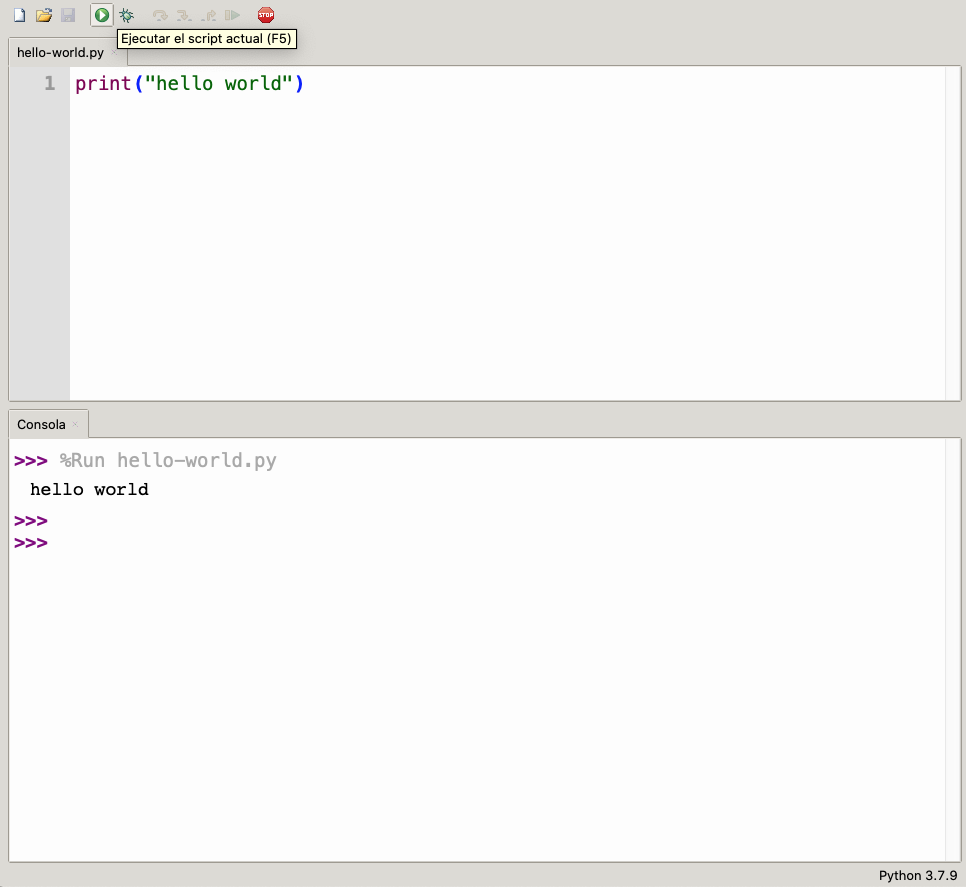
\includegraphics[width=.85\textwidth]{images/Thonny-execute.png}
    \caption{To run: the green arrow button or F5}
    \label{fig:thonny-execute}
\end{figure}


In Figure~\ref{fig:thonny-execute} we see that traditionally, the first program you write in a new programming language is called \verb|hello-world.py| because all it does is show the words \verb|hello world|.  
This is an example of a \textbf{print statement}, although it doesn't actually print anything on paper. This statement displays a result on the screen. In this case, the result is the phrase \verb|hello world| as we can see in the Console after having executed the program.
The quotation marks in the program mark the beginning and the end of the text to be displayed; they do not appear in the result.
\index{comillas}
\index{sentencia!print}
\index{print, sentencia}




In Figure \ref{fig:thonny-execute} we see how we have executed the file \verb|hello-world.py| containing
a program with a single line of code that prints a text string to the screen.

Running a program means calling the Python interpreter and asking it to read the source code
from the \verb|hello-world.py| file, instead of waiting for us to go
entering lines of Python code interactively.

You will notice that there was no need to have \emph{quit()} at the end of the Python program in the file. When Python is reading your source code from a file, it knows to stop when it reaches the end of the file.

\hypertarget{quuxe9-es-un-programa}{%
\section{What is a program?}\label{quuxe9-es-un-programa}}

\begin{definition}
A \textbf{program} at its most basic form is a sequence of statements that have been crafted to do something.
\end{definition}

Even our simple \verb|hello-world.py| script is a program. It is a one-line program and is not particularly useful, but in the strictest definition, it is a Python program.

It might be easiest to understand what a program is by thinking about a problem that a program might be built to solve, and then looking at a program that would solve that problem.

Lets say you are doing Social Computing research on Facebook posts and you are interested in the most frequently used word in a series of posts. You could print out the stream of Facebook posts and pore over the text looking for the most common word, but that would take a long time and be very mistake prone. You would be smart to write a Python program to handle the task quickly and accurately so you can spend the weekend doing something fun.

For example, look at the following text about a clown and a car. Look at the text and figure out the most common word and how many times it occurs.

\begin{verbatim}
    the clown ran after the car and the car ran into the tent
    and the tent fell down on the clown and the car
\end{verbatim}

Then imagine that you are doing this task looking at millions of lines of text. Frankly it would be quicker for you to learn Python and write a Python program to count the words than it would be to manually scan the words.

The even better news is that I already came up with a simple program to find the most common word in a text file.

\begin{python}
name = input('Write the name of the text file: ')
handle = open(name, 'r')
counts = dict()

for line in handle:
    words = line.split()
    for word in words:
        counts[word] = counts.get(word, 0) + 1

bigcount = None
bigword = None
for word, count in list(counts.items()):
    if bigcount is None or count > bigcount:
        bigword = word
        bigcount = count

print("The word: " + bigword)
print("Appears {} times".format(bigcount))
\end{python}


You don't even need to know Python to use this program. You will need to get through Chapter 10 of this book to fully understand the awesome Python techniques that were used to make the program. You are the end user, you simply use the program and marvel at its cleverness and how it saved you so much manual effort. You simply type the code into a file called \verb|words.py| and run it (or you can download the source code directly from PoliformaT). In Poliformat you will also find 5 files, \verb|test1.txt| to \verb|test5.txt|, that you can use to test the program. In Figure \ref{fig:Thonny-execute-words} you can see the result of the first test with the file \verb|test1.txt|, which contains the text of the clown above.

\begin{figure}[t]
    \centering
    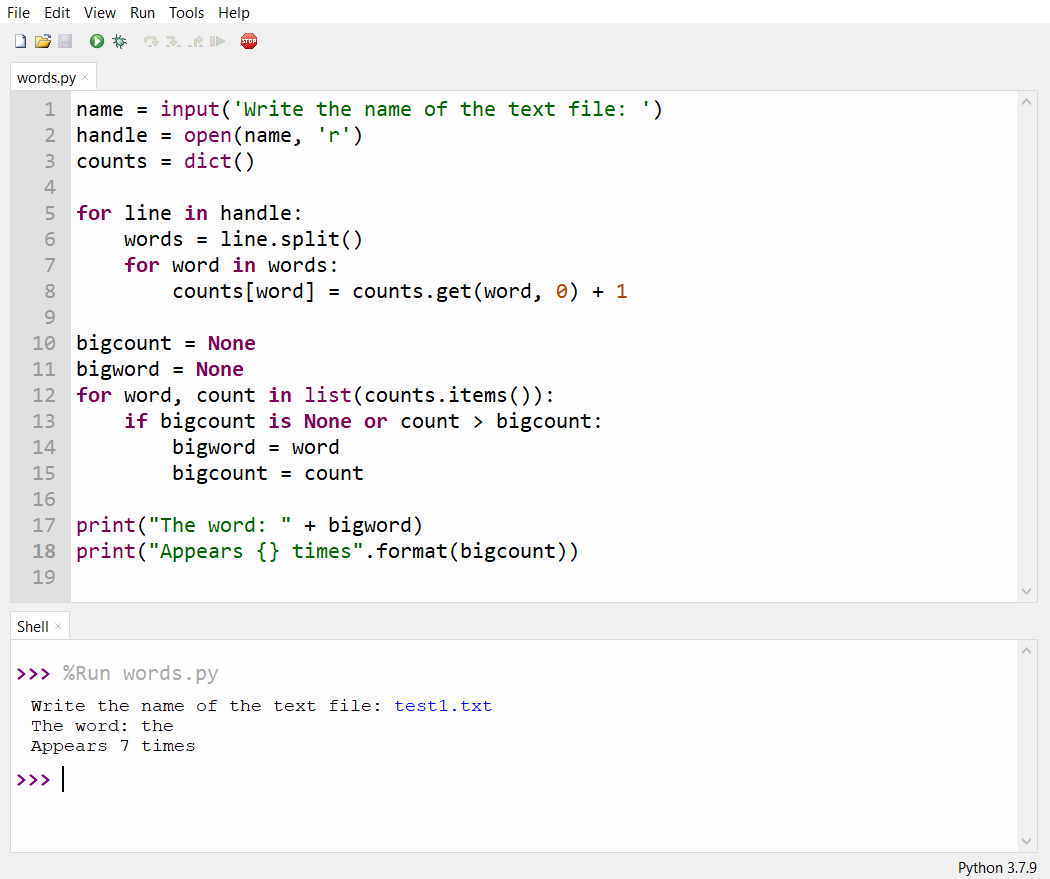
\includegraphics[width=0.85\textwidth]{images/Thonny-execute-words-eng.png}
    \caption{Testing the program}
    \label{fig:Thonny-execute-words}
\end{figure}



\index{programa}
This is a good example of how Python and the Python language are acting as an intermediary between you (the end user) and me (the programmer). Python is a way for us to exchange useful instruction sequences (i.e., programs) in a common language that can be used by anyone who installs Python on their computer. So neither of us are talking to \emph{Python}, instead we are communicating with each other \emph{through} Python.






\hypertarget{los-bloques-de-construction-de-los-programas}{%
\section{The building blocks of programs}\label{los-bloques-de-construction-de-los-programas}}

In the next few chapters, we will learn more about the vocabulary, sentence structure, paragraph structure, and story structure of Python. We will learn about the powerful capabilities of Python and how to compose those capabilities together to create useful programs.

There are some low-level conceptual patterns that we use to construct programs. These constructs are not just for Python programs, they are part of every programming language from machine language up to the high-level languages.

\begin{description}
\tightlist
\item[input]
Get data from the ``outside world''. This might be reading data from a file, or even some kind of sensor like a microphone or GPS. In our initial programs, our input will come from the user typing data on the keyboard.
\item[output]
Display the results of the program on a screen or store them in a file or perhaps write them to a device like a speaker to play music or speak text.
\item[sequential execution]
 Perform statements one after another in the order they are encountered in the \emph{script}.
\item[conditional execution]
Check for certain conditions and then execute or skip a sequence of statements.
\item[repeated execution]
Perform some set of statements repeatedly, usually with some variation.
\item[reuse]
Write a set of instructions once and give them a name and then reuse those instructions as needed throughout your program.
\end{description}

It sounds almost too simple to be true, and of course it is never so simple. It is like saying that walking is simply ``putting one foot in front of the other''. The ``art'' of writing a program is composing and weaving these basic elements together many times over to produce something that is useful to its users.

The word counting program above directly uses all of these patterns except for one.

\hypertarget{quuxe9-cosas-pueden-ir-mal}{%
\section{What could possibly go wrong?}\label{quuxe9-cosas-pueden-ir-mal}}

As we saw in our earliest conversations with Python, we must communicate very precisely when we write Python code. The smallest deviation or mistake will cause Python to give up looking at your program.

Beginning programmers often take the fact that Python leaves no room for errors as evidence that Python is mean, hateful, and cruel. While Python seems to like everyone else, Python knows them personally and holds a grudge against them. Because of this grudge, Python takes our perfectly written programs and rejects them as ``unfit'' just to torment us.

\begin{Verbatim}[frame=single]
>>> primt'Hello, world!'
  File "<pyshell>", line 1
    primt'Hello, world!'
                       ^
SyntaxError: invalid syntax
>>> primt ('Hello, world!')
Traceback (most recent call last):
  File "<pyshell>", line 1, in <module>
NameError: name 'primt' is not defined
>>> I hate you, Python!
  File "<pyshell>", line 1
    I hate you, Python!
      ^
SyntaxError: invalid character in identifier
>>> let's go outside and I will kick your .....
  File "<pyshell>", line 1
    let's go outside and I will kick your .....
           ^
SyntaxError: invalid syntax
>>> 
\end{Verbatim}


There is little to be gained by arguing with Python. It is just a tool. It has no emotions and it is happy and ready to serve you whenever you need it. Its error messages sound harsh, but they are just Python's call for help. It has looked at what you typed, and it simply cannot understand what you have entered.

Python is much more like a dog, loving you unconditionally, having a few key words that it understands, looking you with a sweet look on its face (\texttt{\textgreater{}\textgreater{}\textgreater{}}), and waiting for you to say something it understands. When Python says ``SyntaxError: invalid syntax", it is simply wagging its tail and saying, "You seemed to say something but I just don't understand what you meant, but please keep talking to me
(\texttt{\textgreater{}\textgreater{}\textgreater{}}).''

As your programs become increasingly sophisticated, you will encounter three general types of errors:

\begin{description}
\tightlist
\item[Syntax errors]
These are the first errors you will make and the easiest to fix. A syntax error means that you have violated the "grammar" rules of Python. Python does its best to point right at the line and character where it noticed it was confused. The only tricky bit of syntax errors is that sometimes the mistake that needs fixing is actually earlier in the program than where Python \emph{noticed} it was confused. So the line and character that Python indicates in a syntax error may just be a starting point for your investigation.
\item[Logic errors]
A logic error is when your program has good syntax but there is a mistake in the order of the statements or perhaps a mistake in how the statements relate to one another. A good example of a logic error might be, ``take a drink from your water bottle, put it in your backpack, walk to the library, and then put the top back on the bottle.''
\item[Semantic errors]
A semantic error is when your description of the steps to take is syntactically perfect and in the right order, but there is simply a mistake in the program. The program is perfectly correct but it does not do what you \emph{intended} for it to do. A simple example would be if you were giving a person directions to a restaurant and said, ``\ldots when you reach the intersection with the gas station, turn left and go one mile and the restaurant is a red building on your left''. Your friend is very late and calls you to tell you that they are on a farm and walking around behind a barn, with no sign of a restaurant. Then you say ``did you turn left or right at the gas station?'', and they say, ``I followed your directions perfectly, I have them written down, it says turn left and go one mile at the gas station'', then you say, ``I am very sorry, because while my instructions were syntactically correct, they sadly contained a small but undetected semantic error''.
\end{description}

Again in all three types of errors, Python is merely trying its hardest to do exactly what you have asked.

Syntax errors are encountered by the Python interpreter because it
checks the grammar rules of the language.

Logical and semantic errors can only be found by executing and
testing our program. As we said before, when programming you should always test to ensure that your code does what you expect.

\hypertarget{depurando-los-programas}{%
\section{Testing and debugging of program}\label{depurando-los-programas}}

When we test a program, we run the program to see what comes out and compare this output with what we expect to come out.
%
When Python shows an error or even when it gives you a result that is different from what you had intended, then begins the hunt for the cause of the error. Debugging is the process of finding the cause of the error in your code. When you are debugging a program, and especially if you are working on a hard \emph{bug}, there are four things to try:

\begin{description}
\tightlist
\item[reading]
Examine your code, read it back to yourself, and check that it says what you meant to say.
\item[running]
Experiment by making changes and running different versions. Often if you display the right thing at the right place in the program, the problem becomes obvious, but sometimes you have to spend some time to build scaffolding.
\item[ruminating]
Take some time to think! What kind of error is it: syntax, runtime, semantic? What information can you get from the error messages, or from the output of the program? What kind of error could cause the problem you're seeing? What did you change last, before the problem appeared?
\item[retreating]
At some point, the best thing to do is back off, undoing recent changes, until you get back to a program that works and that you understand. Then you can start rebuilding.
\end{description}

Beginning programmers sometimes get stuck on one of these activities and forget the others. Finding a hard \emph{bug} requires reading, running, ruminating, and sometimes retreating. If you get stuck on one of these activities, try the others. Each activity comes with its own failure mode.

\index{error tipográfico}

For example, reading your code might help if the problem is a typographical error, but not if the problem is a conceptual misunderstanding. If you don't understand what your program does, you can read it 100 times and never see the error, because the error is in your head.

\index{depuración experimental}

Running experiments can help, especially if you run small, simple tests. But if you run experiments without thinking or reading your code, you might fall into a pattern I call ``random walk programming'', which is the process of making random changes until the program does the right thing. Needless to say, random walk programming can take a long time.

\index{programación de paseo aleatorio}
\index{plan de desarrollo!programación de paseo aleatorio}

You have to take time to think. Debugging is like an experimental science. You should have at least one hypothesis about what the problem is. If there are two or more possibilities, try to think of a test that would eliminate one of them.

Taking a break helps with the thinking. So does talking. If you explain the problem to someone else (or even to yourself), you will sometimes find the answer before you finish asking the question.

But even the best debugging techniques will fail if there are too many errors, or if the code you are trying to fix is too big and complicated. Sometimes the best option is to retreat, simplifying the program until you get to something that works and that you understand.

Beginning programmers are often reluctant to retreat because they can't stand to delete a line of code (even if it's wrong). If it makes you feel better, copy your program into another file before you start stripping it down. Then you can paste the pieces back in a little bit at a time.

\hypertarget{el-camino-del-aprendizaje}{%
\section{The learning journey}\label{el-camino-del-aprendizaje}}

As you progress through the rest of the book, don't be afraid if the concepts don't seem to fit together well the first time. When you were learning to speak, it was not a problem for your first few years that you just made cute gurgling noises. And it was OK if it took six months for you to move from simple vocabulary to simple sentences and took 5-6 more years to move from sentences to paragraphs, and a few more years to be able to write an interesting complete short story on your own.

We want you to learn Python much more rapidly, so we teach it all at the same time over the next few chapters. But it is like learning a new language that takes time to absorb and understand before it feels natural. That leads to some confusion as we visit and revisit topics to try to get you to see the big picture while we are defining the tiny fragments that make up that big picture. While the book is written linearly, and if you are taking a course it will progress in a linear fashion, don't hesitate to be very nonlinear in how you approach the material. Look forwards and backwards and read with a light touch. By skimming more advanced material without fully understanding the details, you can get a better understanding of the "why?" of programming. By reviewing previous material and even redoing earlier exercises, you will realize that you actually learned a lot of material even if the material you are currently staring at seems a bit impenetrable.

Usually when you are learning your first programming language, there are a few wonderful ``Ah Hah!'' moments where you can look up from pounding away at some rock with a hammer and chisel and step away and see that you are indeed building a beautiful sculpture.

If something seems particularly hard, there is usually no value in staying up all night and staring at it. Take a break, take a nap, have a snack, explain what you are having a problem with to someone (or perhaps your dog), and then come back to it with fresh eyes. I assure you that once you learn the programming concepts in the book you will look back and see that it was all really easy and elegant and it simply took you a bit of time to absorb it.

\hypertarget{glosario}{%
\section{Glossary}\label{glosario}}

\begin{description}
\tightlist
\item[algorithm]
An algorithm is a sequence of specific instructions of the actions to be carried out and their order to complete a given task. \index{algoritmo}
\item[bug]
An error in a program. \index{bug}
\item[central processing unit]
The heart of any computer. It is what runs the software that we write; also called ``CPU'' or ``the processor''.
\index{unidad central de procesamiento} \index{CPU}
\item[compile]
To translate a program written in a high-level language into a low-level language all at once, in preparation for later execution.
\index{compilar}
\item[high-level language]
A programming language like Python that is designed to be easy for humans to read and write.
\index{lenguaje de alto nivel}
\item[interactive mode]
A way of using the Python interpreter by typing commands and expressions at the prompt.
\index{modo interactivo}
\item[interpret]
To execute a program in a high-level language by translating it one line at a time. \index{interpretar}
\item[low-level language]
A programming language that is designed to be easy for a computer to execute; also called ``machine code'' or ``assembly language''.
\index{lenguaje de bajo nivel}
\item[machine code]
The lowest-level language for software, which is the language that is directly executed by the central processing unit (CPU).
(CPU). \index{código máquina}
\item[main memory]
Stores programs and data. Main memory loses its information when the power is turned off.
\index{memoria principal}
\item[parse]
To examine a program and analyze the syntactic structure.
\index{parsear}
\item[portability]
A property of a program that can run on more than one kind of computer. \index{portabilidad}
\item[print function]
An instruction that causes the Python interpreter to display a value on the screen. \index{print (función)} \index{función!print}
\item[problem solving]
The process of formulating a problem, finding a solution, and expressing the solution. \index{resolución de un problema}
\item[program]
A set of instructions that specifies a computation. \index{programa}
\item[prompt]
When a program displays a message and pauses for the user to type some input to the program. \index{prompt}
\index{indicador de línea de comandos}
\item[secondary memory]
Stores programs and data and retains its information even when the power is turned off. Generally slower than main memory. Examples of secondary memory include disk drives and flash memory in USB sticks.
\index{memoria secundaria}
\item[semantics]
The meaning of a program. \index{semántica}
\item[semantic error]
An error in a program that makes it do something other than what the programmer intended. \index{error semántico}
\item[source code]
A program in a high-level language. \index{código fuente}
\item[test]
Run your program to make sure it does what you expect it to do.
\index{testing}\index{testear}\index{probar}

\end{description}

\hypertarget{ejercicios}{%
\section*{Multiple choice exercises}\label{ejercicios}}
\addcontentsline{toc}{section}{Multiple choice exercises}


\begin{enumerate}
%\setlength{\itemindent}{1.3cm}
\setlength\itemsep{2em}

\item What is the function of the secondary memory in a computer?

a) Execute all of the computation and logic of the program\\
b) Retrieve web pages over the Internet\\
c) Store information for the long term, even beyond a power cycle\\
d) Take input from the user

\item What is a program?

\item What is the difference between a compiler and an interpreter?

\item Which of the following contains "machine code"?

a) The Python interpreter\\
b) The keyboard\\
c) Python source file\\
d) A word processing document


\item  Where in the computer is a variable such as \verb|x| stored after the following Python line finishes?

\begin{Verbatim}[frame=single]
x = 123
\end{Verbatim}

a) Central processing unit\\
b) Main Memory\\
c) Secondary Memory\\
d) Input Devices\\
e) Output Devices

\item What will the following program print out:

\begin{Verbatim}[frame=single]
x = 43
x = x + 1
print(x)
\end{Verbatim}

a) 43\\
b) 44\\
c) x + 1\\
d) Error because x = x + 1 is not possible mathematically

\item Explain each of the following using an example of a human capability:

(1) Central processing unit, 

(2) Main Memory,

(3) Secondary Memory,

(4) Input Device, and

(5) Output Device.

For example, ``What is the human equivalent to a Central Processing Unit''?

\item How do you fix a ``Syntax Error''?

\item  Write a sentence that is semantically understandable but syntactically incorrect. Write another sentence that is syntactically correct but contains semantic errors.

\item Which of the following sentences is correct?

a) In interpretation, each high-level language instruction is translated into machine language, one by one, at runtime.% CORRECT

b) In compilation translates each high-level language instruction one by one into machine language at run time.

c) In interpretation, all the instructions from the language are translated into machine language by means of a program, prior to their execution.

d) Interpretation and compilation are two ways to translate a program written in a machine language into a high-level language.

\end{enumerate}
